\documentclass{article}

\usepackage[utf8]{inputenc}
\usepackage[T1]{fontenc}      
\usepackage[francais]{babel}
\usepackage{graphicx}
\usepackage{circuitikz}
\usepackage[squaren, Gray]{SIunits}
\usepackage{sistyle}
\usepackage[autolanguage]{numprint}
\usepackage{pgfplots}
\pgfplotsset{compat=1.9}
\usepackage{amsmath,amssymb,array}
\usepackage[top=2.5cm,bottom=2.5cm,right=2.5cm,left=2.5cm]{geometry}
\usepackage{url} 
\usepackage{tabularx}
\DeclareMathOperator{\dist}{d}
\newenvironment{abstract-fr}
{
	\begin{center}
		\textbf{Résumé} \\[0.5cm]
	\end{center}
}
{}

\newenvironment{abstract-en}
{
	\begin{center}
		\textbf{Summary} \\[0.5cm]
	\end{center}
}
{}
% New command pour la modélisation mécanique, tri à effectuer
\newcommand\fv[1]{{\bf #1}} % free vector
\newcommand\fvd[1]{\dot{\bf #1}} % free vector derivated
\newcommand\fvdd[1]{\ddot{\bf #1}} % free vector derivated
\newcommand\fvr[1]{\mathring{\bf #1}} % free vector relatively derivated
\newcommand\fvrr[1]{\overset{\circ\circ}{\bf #1}} % free vector relatively derivated
\newcommand\uv[1]{{\bf\hat{ #1}}} % unit vector
\newcommand\ui{{\bf\hat{I}}} % unit vector I
\newcommand\uj{{\bf\hat{J}}} % unit vector J
\newcommand\uk{{\bf\hat{K}}} % unit vector K
\newcommand\wrt[2]{\ensuremath{\tensor*[_{ #1}]{ #2}{}}} % With Respect To
\newcommand\wtr[3]{\ensuremath{\tensor*[_{ #1}]{ #2}{^{ #3}}}} % With Two Respect
\newcommand\omegaf{{\bm \omega}}
\newcommand\omegafr{\mathring{\bm \omega}}
\newcommand\omegafd{\dot{\bm \omega}}
\newcommand\omegaft{\tilde{\bm \omega}}
\newcommand\omegaftr{\mathring{\tilde{\bm \omega}}}
\newcommand\omegat{\tilde{\omega}}
\newcommand\omegatd{\tilde{\dot{\omega}}}
\newcommand\ine{{\bf I}}
\newcommand\st{{\bf L}}
\newcommand\pst{{\bf M}}
\newcommand\lm{{\bf N}}
\newcommand\am{{\bf H}}
\newcommand\amd{\dot{\am}}
\newcommand\fo{{\bf F}}
\newcommand\po{\mathcal{P}}
\newcommand\xg{\ensuremath{\fv{R}}}
\newcommand\xgd{\ensuremath{\fvd{R}}}
\newcommand\xgdd{\ensuremath{\fvdd{R}}}
\newcommand\dvec[1]{\dot{\vec{ #1}}}
\newcommand\ddvec[1]{\ddot{\vec{ #1}}}
\newcommand\qp{\dot{q}}
\newcommand\dqp{\Delta \dot{q}}
\usepackage{url} 
\usepackage{hyperref}
\hypersetup{
    colorlinks,
    citecolor=black,
    filecolor=black,
    linkcolor=black,
    urlcolor=black
}

\begin{document}

\section{Dimensionnement de l'électroaimant et de la bobine mobile}
Pour fabriquer notre haut-parleur, nous ne disposions pas d'aimant permanent. Nous avons donc
dû créer un électroaimant à partir d'un matériau ferromagnétique qui nous a été fourni.
Cette section présente dans un premier temps le dimensionnement de cet électroaimant, c'est-à-dire le
nombre de spires choisi, la résistance totale de la bobine, son inductance, le champ magnétique
induit, etc.

Nous calculerons ensuite, de manière expérimentale, la constante de raideur de la membrane de
notre haut-parleur. A partir de cela et de l'écartement maximal par rapport à sa position d'origine, 
nous pourons calculer la force nécessaire pour déplacer la membrane, et par conséquent, le nombre
de spires nécessaire sur la bobine mobile.

\subsection{Fonctionnement et dimensionnement de la bobine fixe}
Lorsqu'un courant traverse la bobine de cuivre, un champ magnétique est formé.  Nous obtenons 
donc un électroaimant fixe générant le champ nécessaire au déplacement de la seconde bobine. 
C'est cette seconde bobine qui sera responsable du tremblement de la membrane.

\begin{figure}[h]
\centering
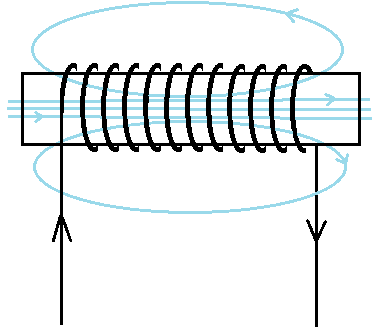
\includegraphics[scale=0.6]{electroaimant.png}
\caption{Modélisation d'un électroaimant}
\label{modélisation de l'électroaimant}
\end{figure}

Le nombre de spires de la bobine fixe, appelons-le $N_1$, a été choisi arbitrairement de manière à produire un
champ magnétique assez fort. Nous avons fixé ce nombre, selon les conseils de notre tuteur, à 500. 
Nous allons maintenant calculer les caractéristiques suivantes de notre électroaimant :

\begin{itemize}
	\item Résistance totale de la bobine ;
	\item Champ magnétique induit ;
	\item Inductance.
\end{itemize}

\paragraph{Résistance totale de la bobine}
Pour calculer la résistance totale de la bobine, nous devons connaître la longueur totale de fil de cuivre utilisé.
Pour cela nous utilisons la formule suivante :

$$L{tot} = N_1 \cdot 2(a + b)$$

Où $N_1 = 500$ est le nombre de spires de la bobine fixe, et $a$ et $b$ sont les longueurs des côtés des spires. Pour
$a = \unit{}{\meter}$ et $b = \unit{}{\meter}$, on trouve :

$$L_{fil} = \unit{}{\meter}$$

Il ne nous reste donc plus qu'à multiplier la longueur totale trouvée par la résistance linéique des fils de cuivre
($R_{lin} = \unit{}{\ohm\per\meter}$) :

$$R = L_{fil} \cdot R_{lin} = \unit{}{\ohm}$$

\paragraph{Champ magnétique induit}
En connaissant la longueur de la bobine $L_{bob}$, le nombre de spires $N_1$, le courant traversant la bobine $I$ et
la perméabilité du matériau $\mu_r$, on peut facilement trouver le champ magnétique induit $B$ à l'intérieur de la bobine 
par la loi d'Ampère :

$$B = \mu_rmu_0I \frac{N_1}{L} = \unit{}{\tesla}$$

Pour $L_{bob} = \unit{}{\meter}$, $\mu_r = 1600$ et $I = \unit{2.5}{\ampere}$.

\paragraph{Inductance de la bobine}
Une fois le champ magnétique induit connu, l'inductance dans la bobine peut être très facilement calculée par :

$$L = N_1 \frac{\phi_B}{I} = \unit{}{\henry}$$

\paragraph{Tableau récapitulatif}

\begin{center}
	\begin{tabular}{c|c|c|c}
		$N_1$ & $B$ & $R$ & $L$ \\
		\hline
		500 & $\unit{}{\tesla}$ & $\unit{}{\ohm}$ & $\unit{}{\henry}$ \\
	\end{tabular}
\end{center}

\subsection{Calcul de la constante de raideur de la membrane}
% TODO

\subsection{Fonctionnement et dimensionnement de la bobine mobile}
% TODO

\paragraph{Calcul du nombre de spires}
En fonction de la constante de raideur de la membrane trouvée dans la sous-section précédente et de l'écartement
maximal de la membrane par rapport à sa position d'origine (fixé à $d = \unit{0.003}{\meter}$), nous sommes en
mesure de trouver le nombre de spires de la bobine mobile $N_2$ :

$$N_2IlB = kx$$

%A continuer

\paragraph{Calcul de la résistance totale de la bobine mobile}
Pour calculer la résistance totale de la bobine, nous devons connaître la longueur totale de fil de cuivre utilisé.
Pour cela nous utilisons la formule suivante :

$$L{tot} = N_2 \cdot 2\pi r$$

Où $N_2 = $ est le nombre de spires de la bobine fixe, et $r$ et le diamètre d'une spire. Pour
$r = \unit{}{\meter}$, on trouve :

$$L_{fil} = \unit{}{\meter}$$

Il ne nous reste donc plus qu'à multiplier la longueur totale trouvée par la résistance linéique des fils de cuivre
($R_{lin} = \unit{}{\ohm\per\meter}$) :

$$R = L_{fil} \cdot R_{lin} = \unit{}{\ohm}$$

\paragraph{Calcul de l'inductance de la bobine mobile}

Une fois le champ magnétique induit connu, l'inductance dans la bobine peut être très facilement calculée par :

$$L = N_1 \frac{\phi_B}{I} = \unit{}{\henry}$$

\paragraph{Tableau récapitulatif}

\begin{center}
	\begin{tabular}{c|c|c|c}
		$N_2$ & $I$ & $R$ & $L$ \\
		\hline
		 $x$ & $\unit{}{\ampere}$ & $\unit{}{\ohm}$ & $\unit{}{\henry}$ \\
	\end{tabular}
\end{center}

\begin{figure}[h]
\centering
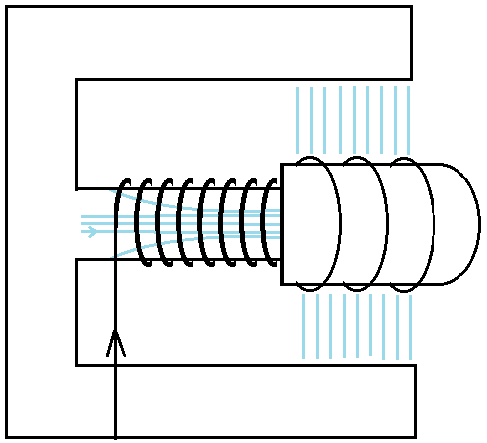
\includegraphics[scale=0.3]{hautparleur.png}
\caption{Vue d'ensemble avec la seconde bobine}
\label{Vue d'ensemble avec la seconde bobine}
\end{figure}

\end{document}
